\documentclass{standalone}
\usepackage[T1]{fontenc}
\usepackage{xcolor}
\usepackage{tikz, pgf-umlcd, xpatch}
\usepackage{amsmath, amssymb}
\usepackage{gradient-text}

\usetikzlibrary{backgrounds}

\definecolor{background}{HTML}{202020}
\definecolor{umlfillcolor}{HTML}{403f40}
\definecolor{umltextcolor}{HTML}{ffffff}
\definecolor{umldrawcolor}{HTML}{f20ae7}
\definecolor{textcolor}{HTML}{ffffff}

\definecolor{void}{HTML}{939393}
\definecolor{private}{HTML}{ff8000}
\definecolor{protected}{HTML}{80c000}
\definecolor{public}{HTML}{00ff00}

\definecolor{virtual}{HTML}{f707bf}
\definecolor{purevirtual}{HTML}{8000ff}
\definecolor{static}{HTML}{0084ff}

\renewcommand{\umlfillcolor}{umlfillcolor}
\renewcommand{\umltextcolor}{umltextcolor}
\renewcommand{\umldrawcolor}{umldrawcolor}

\color[HTML]{ffffff}

\newcommand{\att}[3]{\attribute{#1 #2 : #3 \hfill}}
\newcommand{\op}[4]{\operation{#1 #2(#3) : #4 \hfill}}

\newcommand{\pri}{\color{private}- \color{textcolor}}
\newcommand{\pro}{\color{protected}\# \color{textcolor}}
\newcommand{\pub}{\color{public}+ \color{textcolor}}

\newcommand{\void}{\color{void}void \color{textcolor}}
\newcommand{\variadic}{Args...}
\newcommand{\cstring}{\color[HTML]{079bdb}C-String\color{textcolor}}
\newcommand{\arr}[2]{#1\color{yellow}[\color{textcolor}#2\color{yellow}]\color{textcolor}}

\newcommand{\virtual}[1]{\color{virtual}#1\color{textcolor}}
\newcommand{\purevirtual}[1]{\color{purevirtual}#1\color{textcolor}}
\newcommand{\static}[1]{\color{static}#1\color{textcolor}}

\newcommand{\willchange}[1]{\color{orange}#1\color{textcolor}}




\begin{document}
    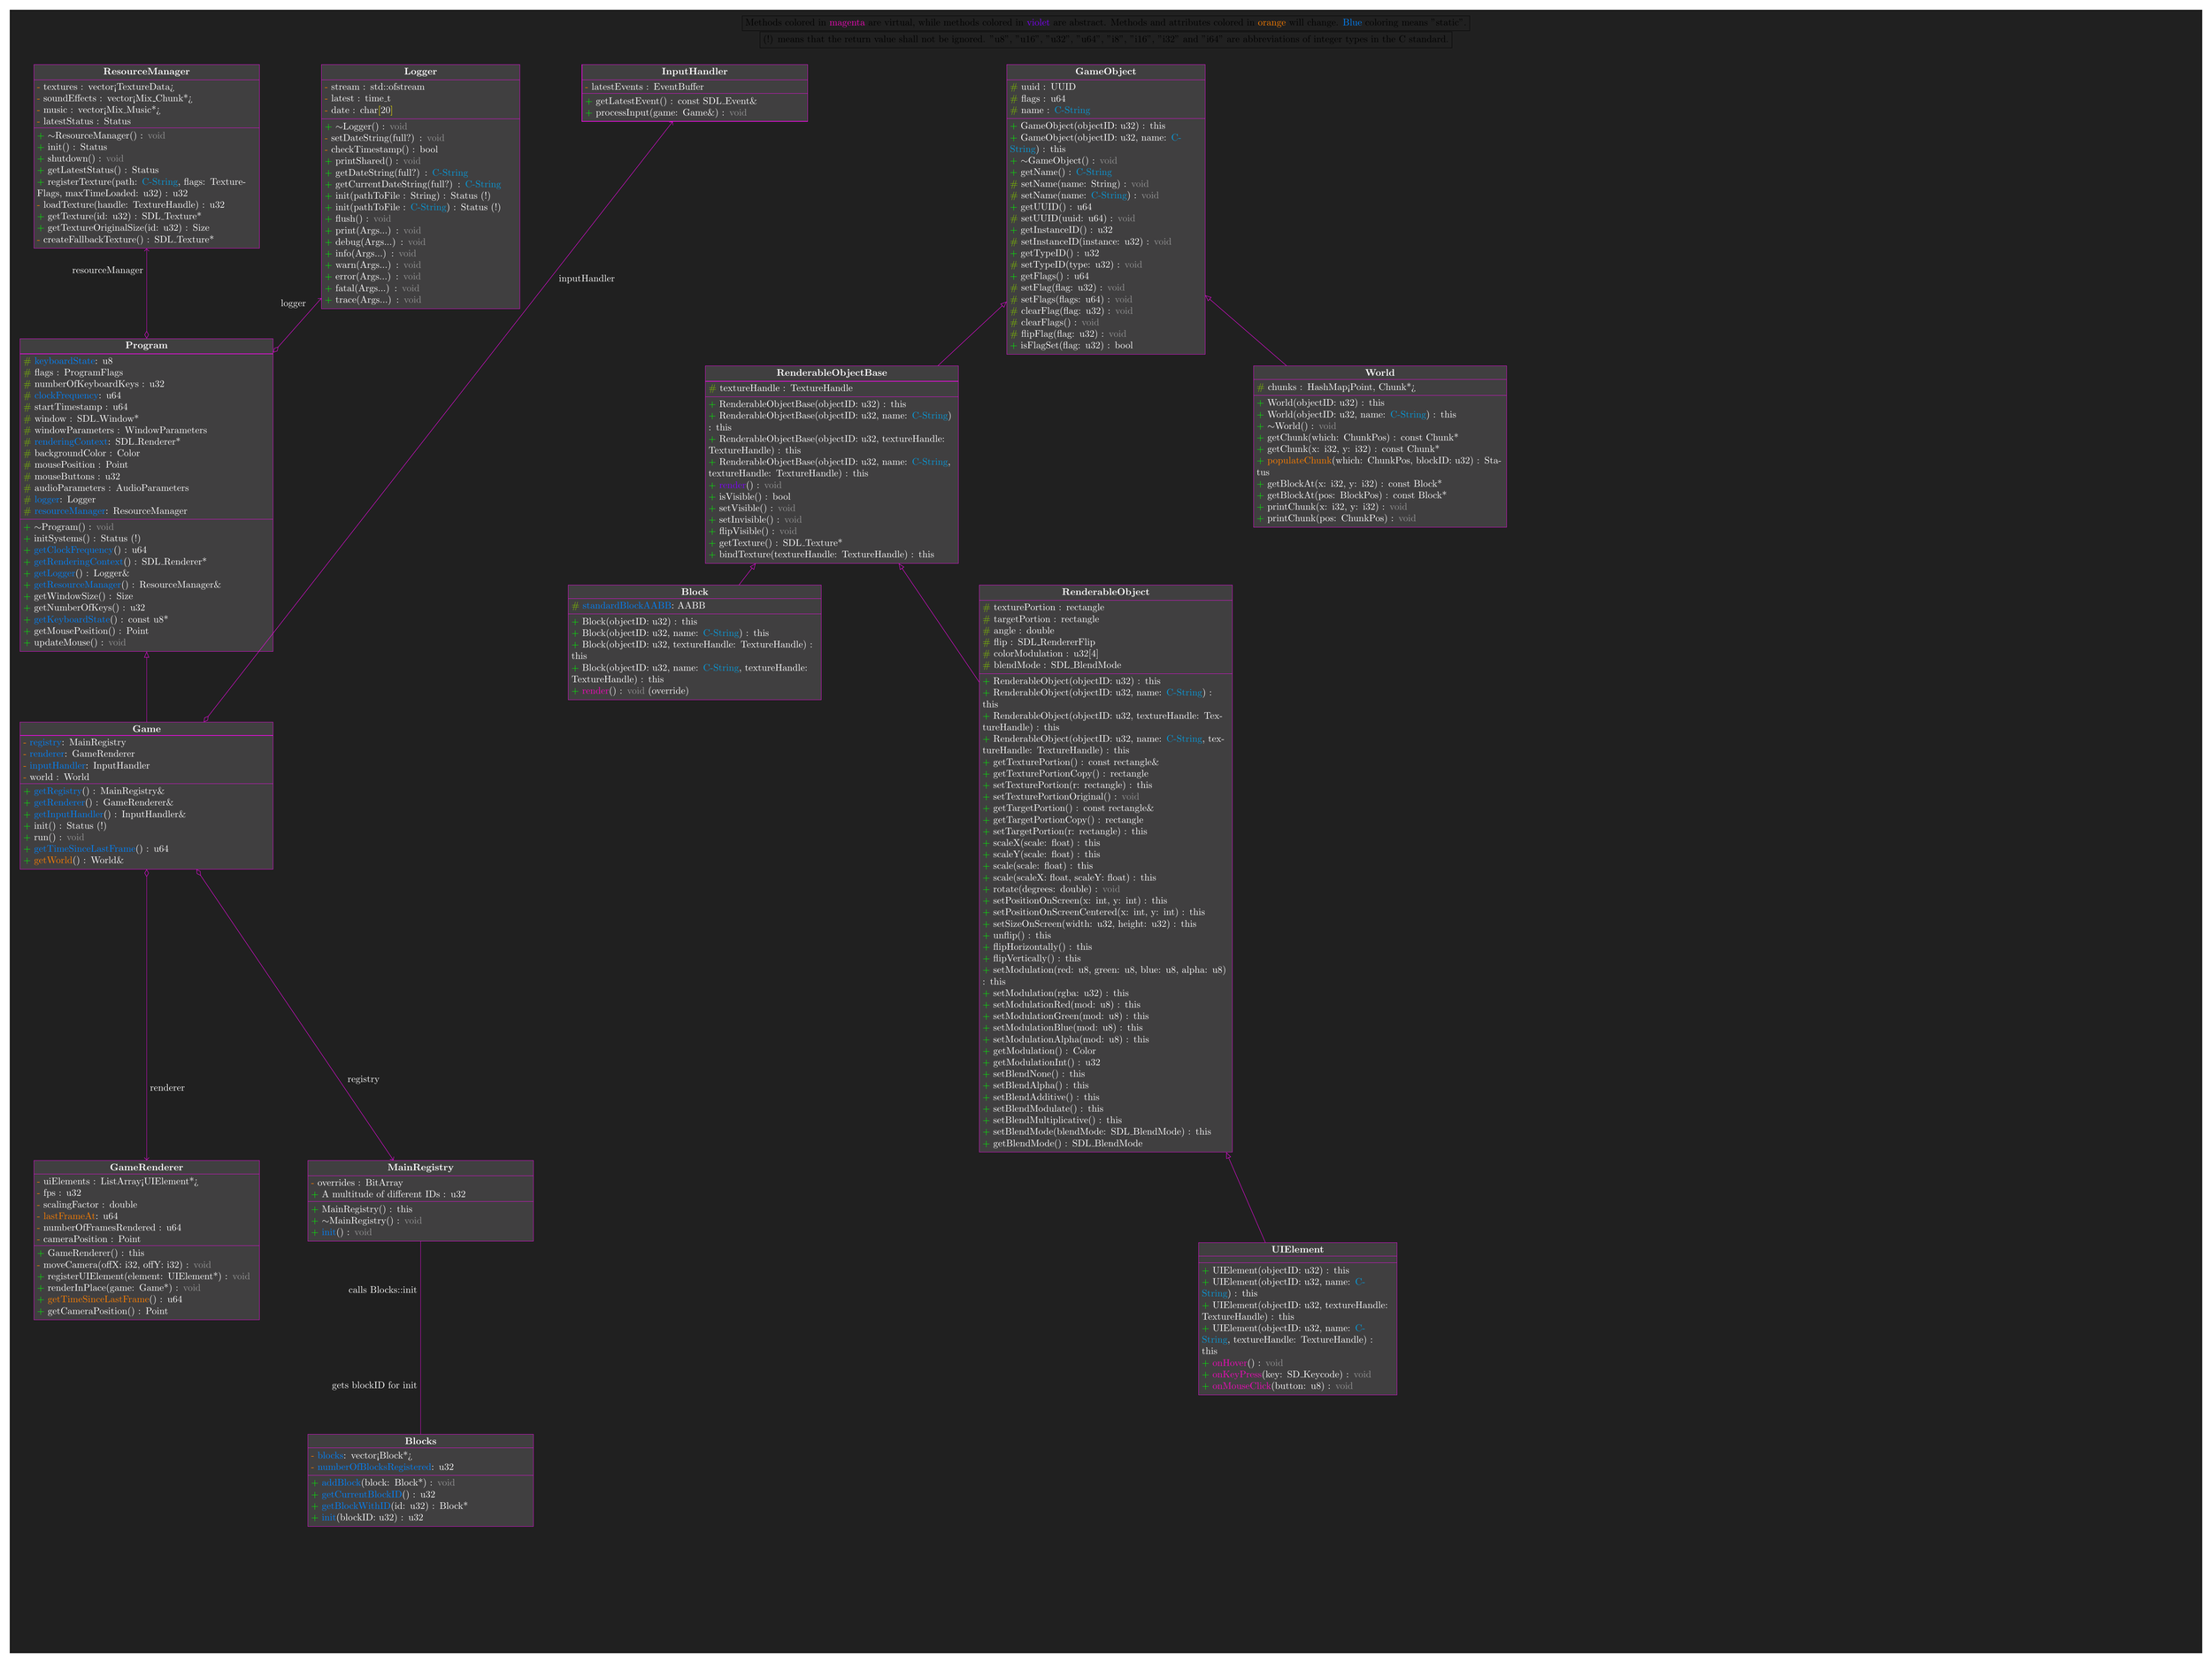
\begin{tikzpicture}
        \node[draw] at (0, 29.5) {
            Methods colored in {\color{virtual}magenta}
            are virtual, while methods colored in
            {\color{purevirtual}violet} are abstract.
            Methods and attributes colored in
            {\color{orange}orange} will change.
            {\color{static}Blue} coloring means "static".

            % Funkcje oznaczone kolorem {\color{virtual}magenta}
            % są wirtualne, a funkcje oznaczone kolorem
            % {\color{purevirtual}fioletowym} są abstrakcyjne.
            % Z kolei funkcje i atrybuty oznaczone kolorem
            % {\color{orange}pomarańczowym} zostaną zmienione.
            % Oznaczenia kolorem {\color{static}niebieskim}
            % oznaczaja statyczność.
        };
        \node[draw] at (0, 28.9) {
            (!) means that the return value shall not be ignored.
            "u8", "u16", "u32", "u64", "i8", "i16", "i32" and "i64"
            are abbreviations of integer types in the C standard.

            % (!) oznacza, że wartość zwrócona nie powinna być zignorowana.
            % "u8", "u16", "u32", "u64", "i8", "i16", "i32" oraz "i64" to skróty
            % od typów liczbowych standardu POSIX.
        };

        

        \begin{scope}[on background layer={color=background}] 
            \fill (-40,-30) rectangle (40,30);
        \end{scope}

        \begin{class}[text width=8cm]{ResourceManager}{-35, 28}
            \att{\pri}{textures}{vector<TextureData>}
            \att{\pri}{soundEffects}{vector<Mix\_Chunk*>}
            \att{\pri}{music}{vector<Mix\_Music*>}
            \att{\pri}{latestStatus}{Status}
            
            \op{\pub}{$\sim$ResourceManager}{}{\void}

            \op{\pub}{init}{}{Status}
            \op{\pub}{shutdown}{}{\void}
            
            \op{\pub}{getLatestStatus}{}{Status}
            
            \op{\pub}{registerTexture}{path: \cstring, flags: TextureFlags, maxTimeLoaded: u32}{u32}
            \op{\pri}{loadTexture}{handle: TextureHandle}{u32}
            
            \op{\pub}{getTexture}{id: u32}{SDL\_Texture*}
            \op{\pub}{getTextureOriginalSize}{id: u32}{Size}
            
            \op{\pri}{createFallbackTexture}{}{SDL\_Texture*}
        \end{class}

        \begin{class}[text width=7cm]{Logger}{-25, 28}
            \att{\pri}{stream}{std::ofstream}
            \att{\pri}{latest}{time\_t}
            \att{\pri}{date}{\arr{char}{20}}

            \op{\pub}{$\sim$Logger}{}{\void}
            \op{\pri}{setDateString}{full?}{\void}
            \op{\pri}{checkTimestamp}{}{bool}            
            \op{\pub}{printShared}{}{\void}
            \op{\pub}{getDateString}{full?}{\cstring}
            \op{\pub}{getCurrentDateString}{full?}{\cstring}
            \op{\pub}{init}{pathToFile : String}{Status (!)}
            \op{\pub}{init}{pathToFile : \cstring}{Status (!)}
            \op{\pub}{flush}{}{\void}
            \op{\pub}{print}{\variadic}{\void}
            \op{\pub}{debug}{\variadic}{\void}
            \op{\pub}{info}{\variadic}{\void}
            \op{\pub}{warn}{\variadic}{\void}
            \op{\pub}{error}{\variadic}{\void}
            \op{\pub}{fatal}{\variadic}{\void}
            \op{\pub}{trace}{\variadic}{\void}
        \end{class}

        \begin{class}[text width=8cm]{InputHandler}{-15, 28}
            \att{\pri}{latestEvents}{EventBuffer}
            
            \op{\pub}{getLatestEvent}{}{const SDL\_Event\&}

            \op{\pub}{processInput}{game: Game\&}{\void}
        \end{class}



        \begin{class}[text width=9cm]{Program}{-35, 18}
            \att{\pro}{\static{keyboardState}}{u8}
            \att{\pro}{flags}{ProgramFlags}
            \att{\pro}{numberOfKeyboardKeys}{u32}
            
            \att{\pro}{\static{clockFrequency}}{u64}
            \att{\pro}{startTimestamp}{u64}

            \att{\pro}{window}{SDL\_Window*}
            \att{\pro}{windowParameters}{WindowParameters}
            \att{\pro}{\static{renderingContext}}{SDL\_Renderer*}
            \att{\pro}{backgroundColor}{Color}
            \att{\pro}{mousePosition}{Point}
            \att{\pro}{mouseButtons}{u32}

            \att{\pro}{audioParameters}{AudioParameters}

            \att{\pro}{\static{logger}}{Logger}
            \att{\pro}{\static{resourceManager}}{ResourceManager}


            \op{\pub}{$\sim$Program}{}{\void}

            \op{\pub}{initSystems}{}{Status (!)}

            \op{\pub}{\static{getClockFrequency}}{}{u64}

            \op{\pub}{\static{getRenderingContext}}{}{SDL\_Renderer*}
            \op{\pub}{\static{getLogger}}{}{Logger\&}
            \op{\pub}{\static{getResourceManager}}{}{ResourceManager\&}

            \op{\pub}{getWindowSize}{}{Size}

            \op{\pub}{getNumberOfKeys}{}{u32}
            \op{\pub}{\static{getKeyboardState}}{}{const u8*}

            \op{\pub}{getMousePosition}{}{Point}
            \op{\pub}{updateMouse}{}{\void}
        \end{class}
        
        \aggregation{Program}{logger}{}{Logger}
        \aggregation{Program}{resourceManager}{}{ResourceManager}


        \begin{class}[text width=8cm]{GameRenderer}{-35, -12}
            \att{\pri}{uiElements}{ListArray<UIElement*>}
            
            \att{\pri}{fps}{u32}
            \att{\pri}{scalingFactor}{double}

            \att{\pri}{\willchange{lastFrameAt}}{u64}
            \att{\pri}{numberOfFramesRendered}{u64}

            \att{\pri}{cameraPosition}{Point}


            \op{\pub}{GameRenderer}{}{this}

            \op{\pri}{moveCamera}{offX: i32, offY: i32}{\void}

            \op{\pub}{registerUIElement}{element: UIElement*}{\void}
            \op{\pub}{renderInPlace}{game: Game*}{\void}

            \op{\pub}{\willchange{getTimeSinceLastFrame}}{}{u64}

            \op{\pub}{getCameraPosition}{}{Point}
        \end{class}

        \begin{class}[text width=8cm]{MainRegistry}{-25, -12}
            \att{\pri}{overrides}{BitArray}
            \att{\pub}{A multitude of different IDs}{u32}

            \op{\pub}{MainRegistry}{}{this}
            \op{\pub}{$\sim$MainRegistry}{}{\void}
            \op{\pub}{\static{init}}{}{\void}
        \end{class}

        \begin{class}[text width=8cm]{Blocks}{-25, -22}
            \att{\pri}{\static{blocks}}{vector<Block*>}
            \att{\pri}{\static{numberOfBlocksRegistered}}{u32}

            \op{\pub}{\static{addBlock}}{block: Block*}{\void}
            
            \op{\pub}{\static{getCurrentBlockID}}{}{u32}
            
            \op{\pub}{\static{getBlockWithID}}{id: u32}{Block*}
            
            \op{\pub}{\static{init}}{blockID: u32}{u32}
        \end{class}

        \association{Blocks}{gets blockID for init}{}{MainRegistry}{calls Blocks::init}{}

        \begin{class}[text width=9cm]{Game}{-35, 4}
            \inherit{Program}

            \att{\pri}{\static{registry}}{MainRegistry}
            \att{\pri}{\static{renderer}}{GameRenderer}
            \att{\pri}{\static{inputHandler}}{InputHandler}

            \att{\pri}{world}{World}


            \op{\pub}{\static{getRegistry}}{}{MainRegistry\&}
            \op{\pub}{\static{getRenderer}}{}{GameRenderer\&}
            \op{\pub}{\static{getInputHandler}}{}{InputHandler\&}

            \op{\pub}{init}{}{Status (!)}

            \op{\pub}{run}{}{\void}

            \op{\pub}{\static{getTimeSinceLastFrame}}{}{u64}

            \op{\pub}{\willchange{getWorld}}{}{World\&}
        \end{class}

        \aggregation{Game}{}{inputHandler}{InputHandler}
        \aggregation{Game}{renderer}{}{GameRenderer}
        \aggregation{Game}{registry}{}{MainRegistry}



        \begin{class}[text width=7cm]{GameObject}{0, 28}
            \att{\pro}{uuid}{UUID}
            \att{\pro}{flags}{u64}
            \att{\pro}{name}{\cstring}

            \op{\pub}{GameObject}{objectID: u32}{this}
            \op{\pub}{GameObject}{objectID: u32, name: \cstring}{this}

            \op{\pub}{$\sim$GameObject}{}{\void}
            
            \op{\pub}{getName}{}{\cstring}
            \op{\pro}{setName}{name: String}{\void}
            \op{\pro}{setName}{name: \cstring}{\void}
            \op{\pub}{getUUID}{}{u64}
            \op{\pro}{setUUID}{uuid: u64}{\void}
            \op{\pub}{getInstanceID}{}{u32}
            \op{\pro}{setInstanceID}{instance: u32}{\void}
            \op{\pub}{getTypeID}{}{u32}
            \op{\pro}{setTypeID}{type: u32}{\void}
            \op{\pub}{getFlags}{}{u64}
            \op{\pro}{setFlag}{flag: u32}{\void}
            \op{\pro}{setFlags}{flags: u64}{\void}
            \op{\pro}{clearFlag}{flag: u32}{\void}
            \op{\pro}{clearFlags}{}{\void}
            \op{\pro}{flipFlag}{flag: u32}{\void}
            \op{\pub}{isFlagSet}{flag: u32}{bool}
        \end{class}

        \begin{class}[text width=9cm]{RenderableObjectBase}{-10, 17}
            \inherit{GameObject}
            
            \att{\pro}{textureHandle}{TextureHandle}

            \op{\pub}{RenderableObjectBase}{objectID: u32}{this}
            \op{\pub}{RenderableObjectBase}{objectID: u32, name: \cstring}{this}
            \op{\pub}{RenderableObjectBase}{objectID: u32, textureHandle: TextureHandle}{this}
            \op{\pub}{RenderableObjectBase}{objectID: u32, name: \cstring, textureHandle: TextureHandle}{this}
            
            \op{\pub}{\purevirtual{render}}{}{\void}

            \op{\pub}{isVisible}{}{bool}
            \op{\pub}{setVisible}{}{\void}
            \op{\pub}{setInvisible}{}{\void}
            \op{\pub}{flipVisible}{}{\void}

            \op{\pub}{getTexture}{}{SDL\_Texture*}
            \op{\pub}{bindTexture}{textureHandle: TextureHandle}{this}
        \end{class}

        \begin{class}[text width=9cm]{World}{10, 17}
            \inherit{GameObject}

            \att{\pro}{chunks}{HashMap<Point, Chunk*>}

            \op{\pub}{World}{objectID: u32}{this}
            \op{\pub}{World}{objectID: u32, name: \cstring}{this}

            \op{\pub}{$\sim$World}{}{\void}

            \op{\pub}{getChunk}{which: ChunkPos}{const Chunk*}
            \op{\pub}{getChunk}{x: i32, y: i32}{const Chunk*}

            \op{\pub}{\willchange{populateChunk}}{which: ChunkPos, blockID: u32}{Status}

            \op{\pub}{getBlockAt}{x: i32, y: i32}{const Block*}
            \op{\pub}{getBlockAt}{pos: BlockPos}{const Block*}

            \op{\pub}{printChunk}{x: i32, y: i32}{\void}
            \op{\pub}{printChunk}{pos: ChunkPos}{\void}
        \end{class}

        \begin{class}[text width=9cm]{RenderableObject}{0, 9}
            \inherit{RenderableObjectBase}

            \att{\pro}{texturePortion}{rectangle}
            \att{\pro}{targetPortion}{rectangle}
            \att{\pro}{angle}{double}
            \att{\pro}{flip}{SDL\_RendererFlip}
            \att{\pro}{colorModulation}{u32[4]}
            \att{\pro}{blendMode}{SDL\_BlendMode}

            \op{\pub}{RenderableObject}{objectID: u32}{this}
            \op{\pub}{RenderableObject}{objectID: u32, name: \cstring}{this}
            \op{\pub}{RenderableObject}{objectID: u32, textureHandle: TextureHandle}{this}
            \op{\pub}{RenderableObject}{objectID: u32, name: \cstring, textureHandle: TextureHandle}{this}
            
            \op{\pub}{getTexturePortion}{}{const rectangle\&}
            \op{\pub}{getTexturePortionCopy}{}{rectangle}
            \op{\pub}{setTexturePortion}{r: rectangle}{this}
            \op{\pub}{setTexturePortionOriginal}{}{\void}

            \op{\pub}{getTargetPortion}{}{const rectangle\&}
            \op{\pub}{getTargetPortionCopy}{}{rectangle}
            \op{\pub}{setTargetPortion}{r: rectangle}{this}

            \op{\pub}{scaleX}{scale: float}{this}
            \op{\pub}{scaleY}{scale: float}{this}
            \op{\pub}{scale}{scale: float}{this}
            \op{\pub}{scale}{scaleX: float, scaleY: float}{this}

            \op{\pub}{rotate}{degrees: double}{\void}

            \op{\pub}{setPositionOnScreen}{x: int, y: int}{this}
            \op{\pub}{setPositionOnScreenCentered}{x: int, y: int}{this}
            \op{\pub}{setSizeOnScreen}{width: u32, height: u32}{this}

            \op{\pub}{unflip}{}{this}
            \op{\pub}{flipHorizontally}{}{this}
            \op{\pub}{flipVertically}{}{this}

            \op{\pub}{setModulation}{red: u8, green: u8, blue: u8, alpha: u8}{this}
            \op{\pub}{setModulation}{rgba: u32}{this}
            \op{\pub}{setModulationRed}{mod: u8}{this}
            \op{\pub}{setModulationGreen}{mod: u8}{this}
            \op{\pub}{setModulationBlue}{mod: u8}{this}
            \op{\pub}{setModulationAlpha}{mod: u8}{this}
            \op{\pub}{getModulation}{}{Color}
            \op{\pub}{getModulationInt}{}{u32}

            \op{\pub}{setBlendNone}{}{this}
            \op{\pub}{setBlendAlpha}{}{this}
            \op{\pub}{setBlendAdditive}{}{this}
            \op{\pub}{setBlendModulate}{}{this}
            \op{\pub}{setBlendMultiplicative}{}{this}
            \op{\pub}{setBlendMode}{blendMode: SDL\_BlendMode}{this}
            \op{\pub}{getBlendMode}{}{SDL\_BlendMode}
            
        \end{class}

        \begin{class}[text width=9cm]{Block}{-15, 9}
            \inherit{RenderableObjectBase}

            \att{\pro}{\static{standardBlockAABB}}{AABB}

            \op{\pub}{Block}{objectID: u32}{this}
            \op{\pub}{Block}{objectID: u32, name: \cstring}{this}
            \op{\pub}{Block}{objectID: u32, textureHandle: TextureHandle}{this}
            \op{\pub}{Block}{objectID: u32, name: \cstring, textureHandle: TextureHandle}{this}
            
            \op{\pub}{\virtual{render}}{}{\void (override)}
        \end{class}

        \begin{class}[text width=7cm]{UIElement}{7, -15}
            \inherit{RenderableObject}

            \op{\pub}{UIElement}{objectID: u32}{this}
            \op{\pub}{UIElement}{objectID: u32, name: \cstring}{this}
            \op{\pub}{UIElement}{objectID: u32, textureHandle: TextureHandle}{this}
            \op{\pub}{UIElement}{objectID: u32, name: \cstring, textureHandle: TextureHandle}{this}
            
            \op{\pub}{\virtual{onHover}}{}{\void}
            \op{\pub}{\virtual{onKeyPress}}{key: SD\_Keycode}{\void}
            \op{\pub}{\virtual{onMouseClick}}{button: u8}{\void}
        \end{class}
        
    \end{tikzpicture}
\end{document}